\documentclass[a4paper,french]{paper}
\usepackage{../../../../../_assets/latex/5N_OPTO_ELEC}

%Informations about this document 
%------------------------------------------
\def\module{Opto-Electronique - S5}
\def\moduleAbrege{5N-027-SCI / OptoElec}
\def\annee{2024-2025}

\def\titre{Séance 3 / Filtrage d'un signal électrique}
\author{Julien VILLEMEJANE}

\subtitle{Séance 3}
\institution{LEnsE / Institut d'Optique Graduate School}

\title{\titre}
\begin{document} 
%Beginning First Page. 
%------------------------------------------
\enteteThematiqueObligatoire{}

\textit{Pour ce TD, on pourra s'appuyer sur les fiches résumées} : \href{https://lense.institutoptique.fr/ressources/Annee1/Electronique/fiches/2020_FR_RegimeHarmonique.pdf}{Régime Harmonique}, \href{https://lense.institutoptique.fr/ressources/Annee1/Electronique/fiches/2021_FR_ALI.pdf}{Ampli Linéaire Intégré} et \href{https://lense.institutoptique.fr/ressources/Annee1/Electronique/fiches/2020_FR_FiltreOrdre1.pdf}{Filtre d'ordre 1}

%Beginning Content. 
%------------------------------------------

%%%%%%%%%%%%%%%%%%%
%%%%%%%%%%%%%%%%%%%
\encadreTDExo{3.1 - Charge et décharge d'un condensateur}{

Soit le circuit suivant :

\begin{center}
\begin{circuitikz}
	\draw (0,0) to [R=$R$, o-*] (3,0)
		to[C=$C$, -*] (3,-3)
		to[short, -*](1,-3)
		node[ground](GND){}
		to[short, -o](0,-3);
	\draw (3,0) to[short, -o](4,0);
	\draw (3,-3) to[short, -o](4,-3);
	% fleche
	\draw (0,-2.7) edge[->] (0,-0.3);
	\node (Ein) at (-0.5,-1.5){$V_E$};
	% fleche
	\draw (4,-0.3) edge[<-, green!40!black] (4,-2.7); 
	\node[text=green!40!black] (US) at (4.5,-1.5){$V_S$};
\end{circuitikz}
\end{center}

\begin{enumerate}
	\item Donnez le lien entre $V_E(t)$ et $V_S(t)$.
	\item Donnez l'expression de $V_S(t)$ pour $t > 0$ pour $V_E(t) = E$ (constante). On supposera le condensateur totalement déchargé à $t = 0$ (c'est à dire si $V_S(0) = 0$) et tracez $V_S(t)$.
	\item Donnez le protocole de mesure de la \textbf{réponse indicielle} de ce circuit. 
\end{enumerate}
}

%%%%%%%%%%%%%%%%%%%

\textbf{Question 1}

La loi des mailles donne : $V_E(t) - R \cdot i(t) - V_S(t) = 0$ et la caractéristique d'un condensateur donne : $i(t) = C \cdot \frac{d V_S(t)}{d t}$.

En effet, pour un condensateur : $q = C \cdot V_S (t)$ et le courant associé vaut alors $i = \frac{d q}{d t}$

Ainsi : 

$$V_E(t) = R \cdot C \cdot \frac{d V_S(t)}{d t} + V_S(t)$$

\centerline {\rule{.5\linewidth}{.25pt}} % Horizontal line

\textbf{Question 2}

a) On cherche les solutions de l'équation homogène : $$\frac{d V_S(t)}{d t} + \frac{1}{R \cdot C} \cdot V_S(t) = 0$$

Ces solutions sont de la forme : $V_{S0}(t) = k \cdot exp(\frac{-t}{R \cdot C})$ avec $k \in \mathbb{R}$

b) On cherche une solution particulière de la même forme que le second membre. Dans notre cas, $E/RC$ qui est une constante.

Si $V_{S1}(t) = m$, alors $\frac{d V_{S1}(t)}{d t} = 0$.

On a alors, en reprenant l'équation initiale : $\frac{m}{R \cdot C} = \frac{E}{R \cdot C}$. Ainsi $m = E$.

c) Les solutions de l'équation sont alors la somme des deux solutions précédentes. Ainsi : $$V_S(t) = V_{S0}(t) + V_{S1}(t) = k \cdot exp(\frac{-t}{R \cdot C} + E$$

d) On obtient ensuite $k$ en utilisant la condition initiale, à savoir $V_S(0) = 0$. Ainsi $k = -E$.

On obtient alors l'expression suivante pour $V_s(t)$ :

$$V_S(t) = E \cdot (1 - exp(\frac{-t}{R \cdot C})$$

\begin{center}
	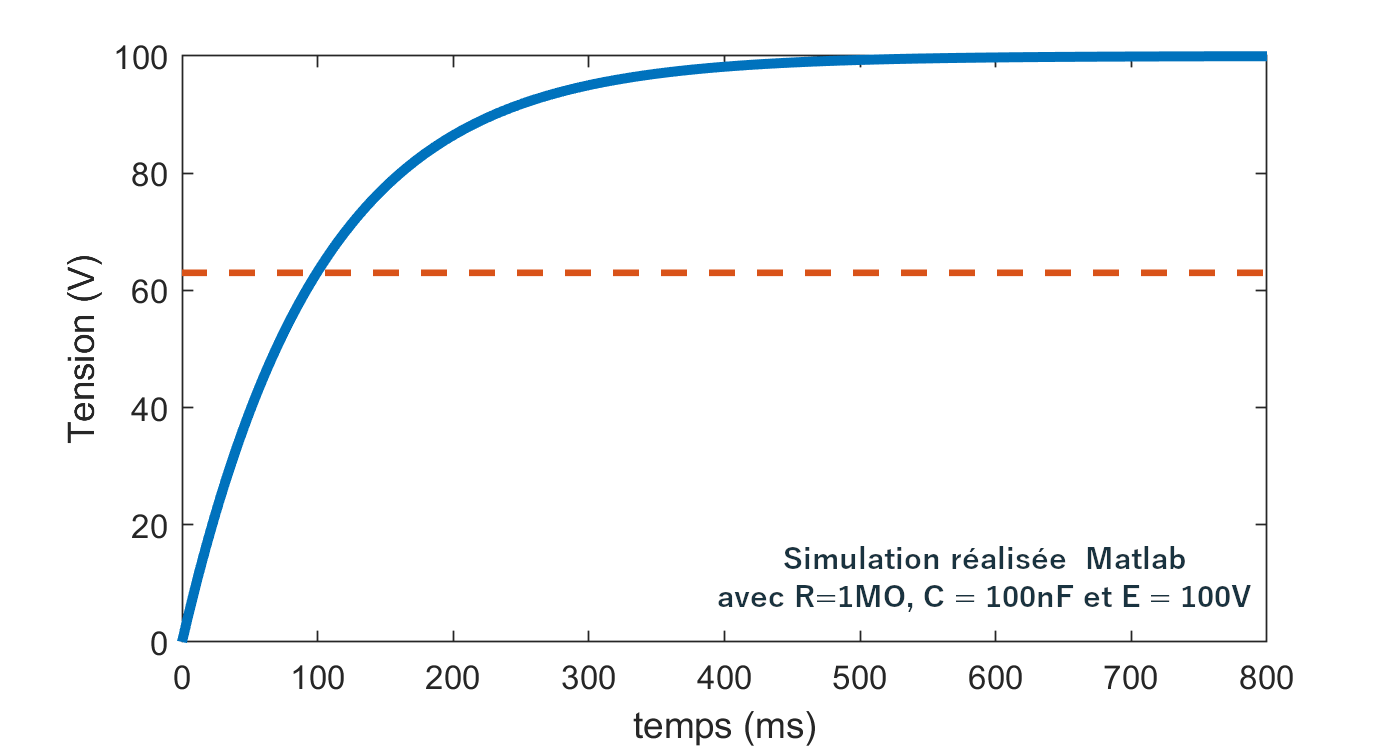
\includegraphics[width=8cm]{images/syst_ordre1_003_a_corr.png}
\end{center}

\centerline {\rule{.5\linewidth}{.25pt}} % Horizontal line

\textbf{Question 3}

Pour mesurer la réponse indicielle (ou réponse à un échelon) de ce circuit, il faut utiliser : 
\begin{itemize}
	\item un générateur de signaux basse fréquence (GBF), appliquant un signal carré de grande période ($T >> R \cdot C$) et d'amplitude d'environ $1\operatorname{V}$ sur l'entrée $V_e(t)$ ;
	\item un oscilloscope permettant de visualiser à la fois $V_e(t)$ (canal 1 et synchronisé sur ce signal) et $V_s(t)$.
\end{itemize}


%%%%%%%%%%%%%%%%%%%
%%%%%%%%%%%%%%%%%%%
\encadreTDExo{3.2 - Filtre analogique d'ordre 1}{

On reprend le schéma de l'exercice précédent (exercice 3.1), mais cette fois-ci, nous nous plaçons dans un régime harmonique. Ce circuit est alors alimenté par une source de tension sinusoïdale de pulsation $\omega_0$. On prendra $R = 1\operatorname{M\Omega}$ et $C = 100\operatorname{nF}$.

\begin{enumerate}
	\item Déterminez la \textbf{fonction de transfert} $T( j\omega ) = V_s / V_e$ en fonction de la pulsation et des éléments du montage.
		
	\item Déduisez la \textbf{pulsation de coupure} $\omega_0$ de $T( j\omega )$ et le \textbf{gain dans la bande-passante} en fonction des éléments du montage.

	\item Tracez le \textbf{diagramme de Bode} du gain et de la phase en fonction de la pulsation.

	\medskip
	
	On réalise la réponse en fréquence de ce système expérimentalement à l'aide d'un générateur de fonction ($R_s = 50\operatorname{\Omega}$) et d'un oscilloscope numérique ($R_e = 1\operatorname{M\Omega}$).
	
	Après analyse, nous obtenons une fréquence caractéristique $\omega_c = 20\operatorname{rd/s}$ et une amplification dans la bande passante de 0.5.
	
	\item Proposez une explication à ces résultats.
	
	\medskip
	
	\item On met deux étages de ce type en \textbf{cascade}. Quelle est la fonction de transfert alors obtenue ?

\end{enumerate}
}

%%%%%%%%%%%%%%%%%%%
\textbf{Question 1}

En appliquant un seul signal sinusoïdal sur ce circuit, on peut alors se placer en régime harmonique et ainsi utiliser les notations complexes. En régime harmonique, l'ensemble des lois fondamentales de la physique peuvent s'appliquer : loi des mailles, loi d'Ohm, superposition...

Ainsi, on a $V_E = R \cdot I + Z_C \cdot I$ avec $Z_C = \frac{1}{j \cdot R \cdot C \cdot \omega}$

On obtient alors : $$I = \frac{j \cdot C \cdot \omega}{1 + j \cdot R \cdot C \cdot \omega} \cdot V_E$$

On a : $V_S = Z_C \cdot I$.

On obtient alors la relation suivante : $$V_S = \frac{1}{1 + j \cdot R \cdot C \cdot \omega} \cdot V_E$$

Ainsi, la fonction de transfert que l'on obtient est la suivante :

$$T(j\cdot\omega) = \frac{V_S}{V_E} = \frac{1}{1 + j \cdot R \cdot C \cdot \omega}$$

\centerline {\rule{.5\linewidth}{.25pt}} % Horizontal line
%%%%%%%%%%%%%%%%%%%
\textbf{Question 2}

On peut alors mettre cette expression sous la forme normalisée d'un système passe-bas du premier ordre : $T(j\cdot\omega) = \frac{T_0}{1 + j \cdot \frac{\omega}{\omega_0}}$. 

On obtient par identification à l'expression obtenue précédemment : $\omega_0 = \frac{1}{R \cdot C}$ et $T_0 = 1$.

L'application numérique donne $\omega_0 = 10\operatorname{rd/s}$ soit une fréquence $f_0 = 1.59\operatorname{Hz}$.


\centerline {\rule{.5\linewidth}{.25pt}} % Horizontal line
%%%%%%%%%%%%%%%%%%%
\textbf{Question 3}

Pour tracer le diagramme de Bode de ce circuit, on s'intéresse au module de la fonction de transfert et à la phase de celle-ci.

Pour simplifier les calculs par la suite, on préfère utiliser le gain (en dB) de cette fonction de transfert : $G = 20 \cdot \log{}(\lvert T \rvert)$

On obtient alors le diagramme de Bode suivant :

\begin{center}
	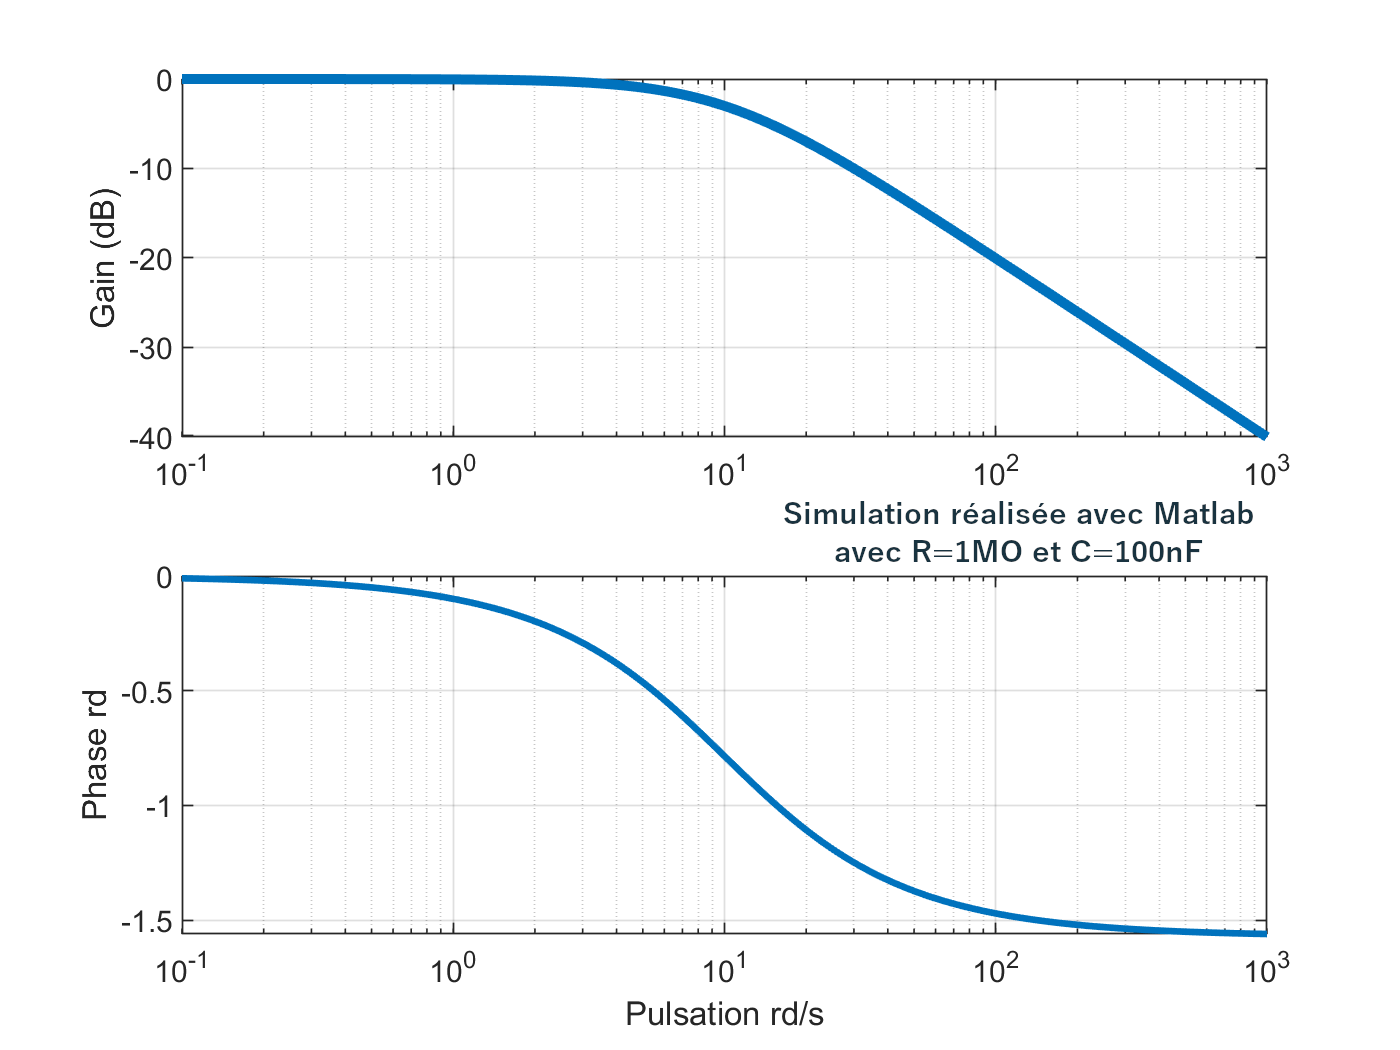
\includegraphics[width=8cm]{images/syst_ordre1_003_b_corr.png}
\end{center}

Obtenu à l'aide du programme MatLAB suivant :

\begin{lstlisting}[style=Matlab-editor]
R = 1e6;
C = 1e-7;
% Vecteur des pulsations de $10^1$ a $10^5$ sur 101 points
w = logspace(1,5,1001);

% TF du circuit
T = 1 ./ (1 + 1j * R * C * w);

% Bode en echelle logarithmique
figure;
subplot(2,1,1);
semilogx(w, 20*log10(abs(T)));
grid on;
ylabel('Gain (dB)');
subplot(2,1,2);
semilogx(w, angle(T));
ylabel('Phase rd');
xlabel('Pulsation rd/s');
\end{lstlisting}

\textbf{Complément d'informations}

La \textbf{réponse fréquentielle} $H(f) = V_S(f) / V_E(f)$ d'un système permet de connaitre, \textbf{quelque soit la fréquence $f$ du signal d'entrée} : 
\begin{itemize}
	\item l'\textbf{amplitude du signal de sortie} en fonction de celle du signal d'entrée,
	\item le déphasage du signal de sortie par rapport au signal d'entrée.
\end{itemize}

Il est \textbf{théoriquement nécessaire de tester l'ensemble des fréquences du spectre} et de mesurer l'amplitude du signal de sortie et du signal d'entrée ainsi que la phase entre ces deux signaux.

\medskip

\textbf{Mais quel signal faut-il pour réaliser ces mesures ?}

On cherche à mesurer $H(f)$ (dans l'\textbf{espace des fréquences}) pour toutes les fréquence $f$ disponibles. Cependant, nous ne pouvons effectuer nos relevés que dans l'\textbf{espace temporel}. Il serait donc intéressant d'utiliser un signal de fréquence unique $f_0$ tel que la transformée de Fourier de ce signal permette d'obtenir $H(f_0)$ (ou une image de $H(f_0)$). 

On rappelle que $V_S(f) = H(f) \cdot V_E(f)$ dans l'espace fréquentiel, et $v_s(t) = h(t) \ast v_e(t)$ dans l'espace temporel.

\medskip

Si $v_e(t) = A \cdot \sin{}(2 \cdot \pi \cdot f \cdot t)$, alors sa transformée de Fourier vaut : $V_E(f) = \frac{A}{2} \cdot (\delta(-f_0) + \delta(f_0)) $

Ainsi, on obtient en sortie du système : $V_S(f) = H(f) \cdot A \cdot \delta(f_0) = A \cdot H(f_0)$

\centerline {\rule{.5\linewidth}{.25pt}} % Horizontal line
%%%%%%%%%%%%%%%%%%%
\textbf{Question 4} 
	
Les appareils d'instrumentation permettant de réaliser les mesures (ici un GBF et un oscilloscope) ne sont pas parfaits. Il est alors possible de modéliser le montage de la façon suivante :

\begin{center}
	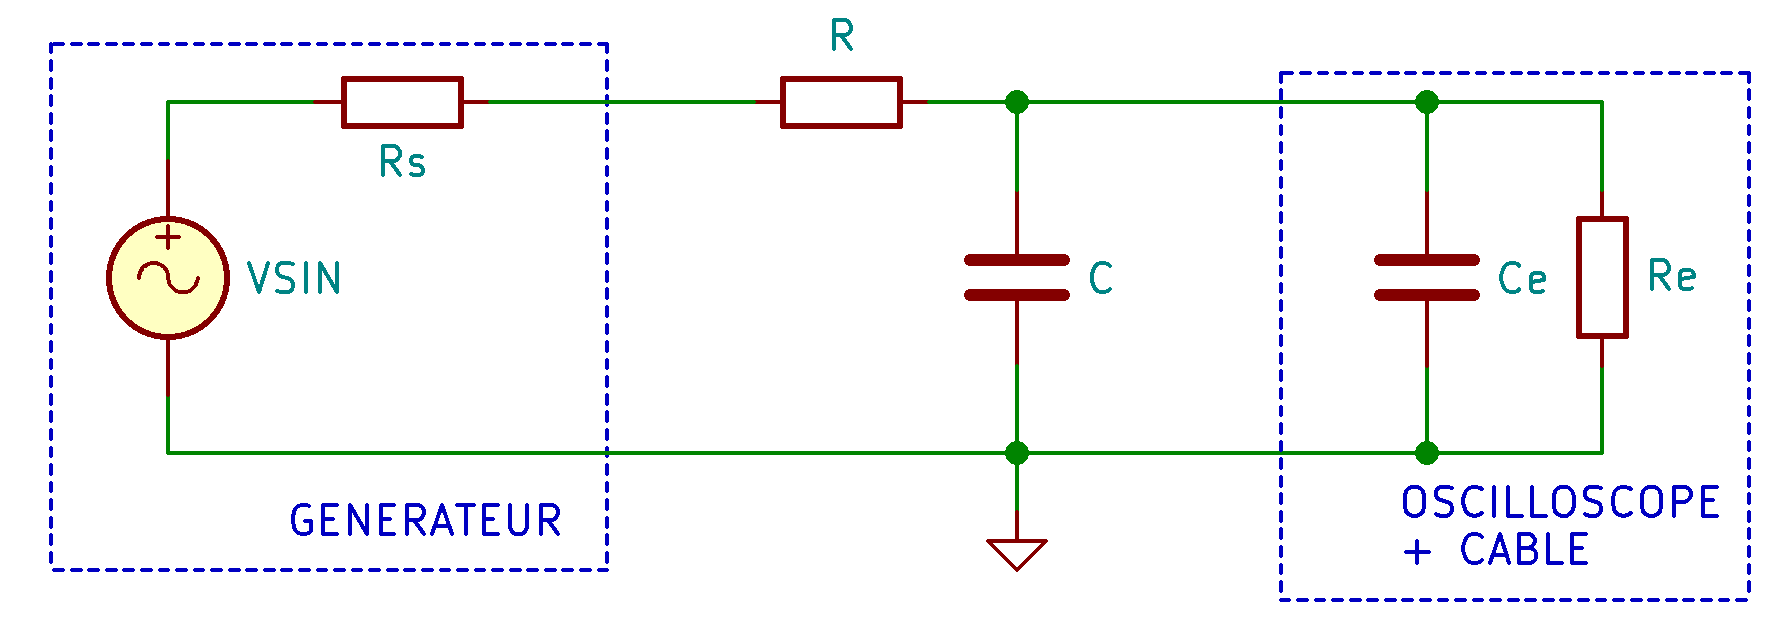
\includegraphics[width=8cm]{images/caract_002_corr.png}
\end{center}

Côté GBF, la tension appliquée (et paramètrée) par le GBF n'est pas tout à fait $V_e$. En effet, l'impédance de sortie du générateur n'est pas nulle (comme elle devrait l'être idéalement). On peut la négliger dans la plupart des cas, car cette dernière vaut en général $50\Omega$.

Côté oscilloscope, nous allons nous intéresser à son impédance d'entrée. Elle est la plupart des cas de $1M\Omega$.

Si on reprend le calcul de la fonction de transfert en prenant en compte l'impédance d'entrée $R_e$ de l'oscilloscope, on obtient alors : 

$$\frac{V_S}{V_e} = \frac{Z_q}{Z_q + R}$$ avec $Z_q = R_e // C = \frac{R_e}{1 + j \cdot R_e \cdot C \cdot \omega}$.

Après simplification, on obtient : 

$$\frac{V_S}{V_e} = \frac{R_e}{R + R_e} \cdot \frac{1}{1 + j \cdot \frac{R \cdot R_e}{R + R_e} \cdot C \cdot \omega}$$

Par identification avec l'expression normalisée d'un filtre du premier ordre, on obtient : $T_0 = \frac{R_e}{R + R_e}$ et $\omega_0 = \frac{R + R_e}{R \cdot R_e \cdot C}$.

\centerline {\rule{.5\linewidth}{.25pt}} % Horizontal line
%%%%%%%%%%%%%%%%%%%
\textbf{Question 5} 

On appelera $V_{S1}$ la sortie du premier étage et $V_{S2}$ celle du second étage.

$V_{S2} = V_{S1} \cdot \frac{1}{1 + j \cdot R \cdot C \cdot \omega}$ (d'après les questions précédentes).

Pour calculer la tension $V_{S1}$, on peut utiliser le théorème de Millman.

On obtient alors : $$V_{S1} = \frac{\frac{V_e}{R} + \frac{V_{S2}}{R}}{\frac{2}{R} + j \cdot C \cdot \omega}$$

Après simplification, on obtient : $$\frac{V_{S2}}{V_e} = \frac{1}{(1 + j \cdot R \cdot C \cdot \omega) \cdot (2 + j \cdot R \cdot C \cdot \omega) - 1}$$

\medskip

Cette fonction de transfert est différente de $T(j \omega)^2 = (\frac{1}{1 + j \cdot R \cdot C \cdot \omega})^2$. La simulation suivante permet de comparer les 3 fonctions de transfert suivantes : celle du premier ordre, celle de la mise en cascade et celle du premier ordre au carré.

\begin{center}
	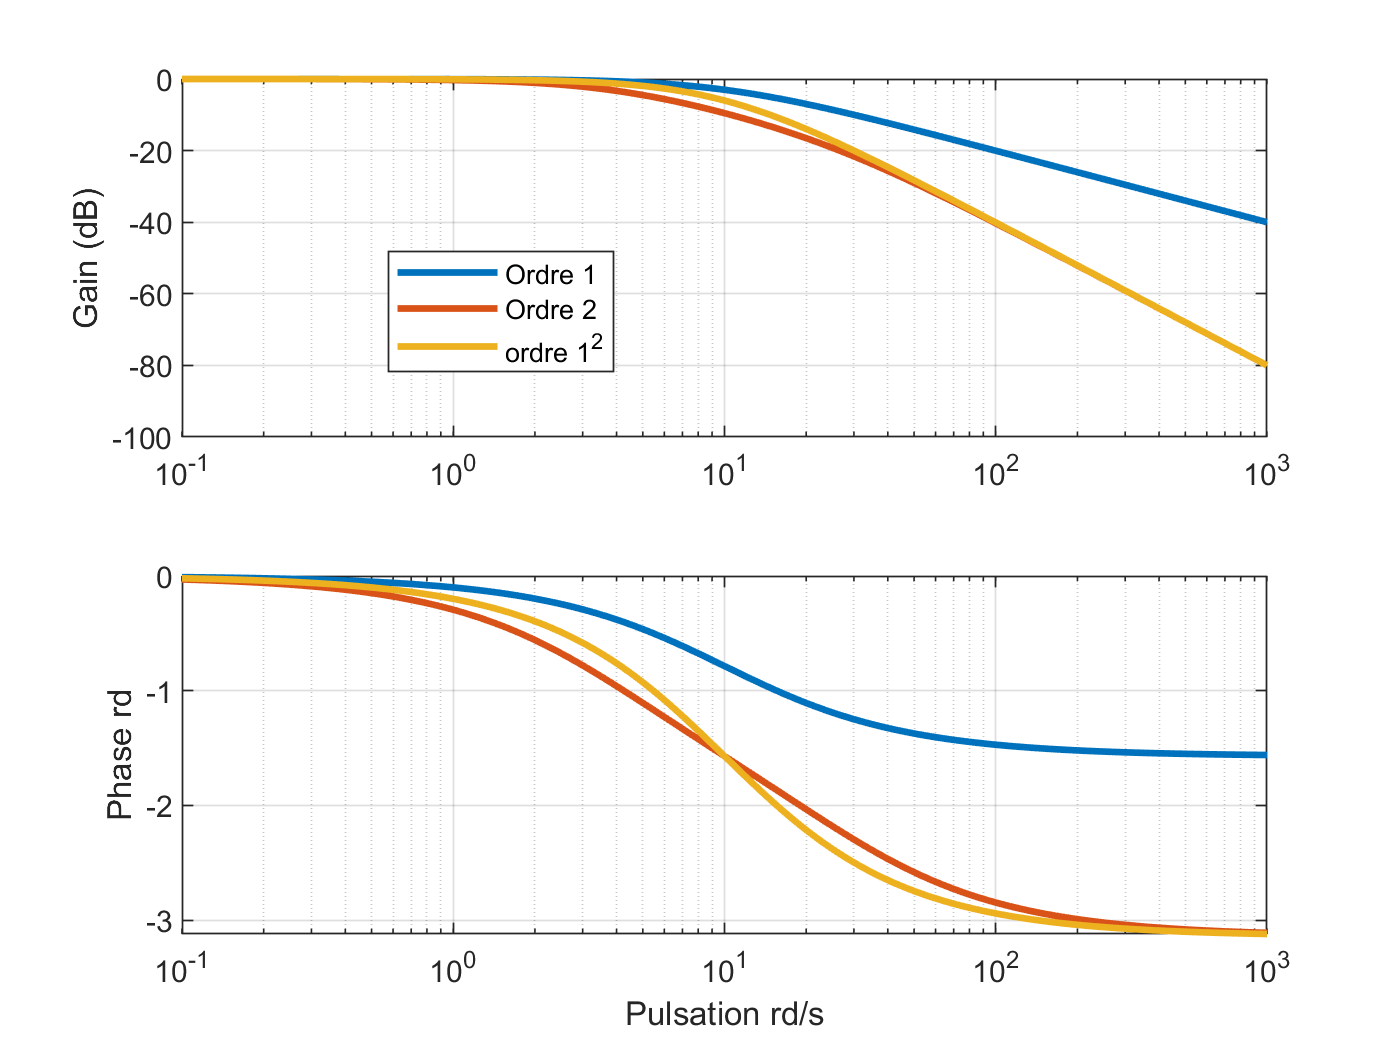
\includegraphics[width=8cm]{images/syst_ordre1_004_b_corr.png}
\end{center}



%%%%%%%%%%%%%%%%%%%
%%%%%%%%%%%%%%%%%%%
\encadreTDExo{3.3 - Filtre universel}{

%%%%%%%%%%%%%%%%%%%
\textbf{Bloc intégrateur}

On se propose d'étudier la réponse du système suivant :

\begin{center}
	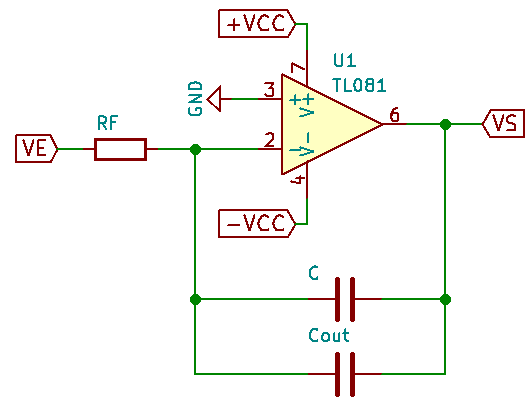
\includegraphics[width=8cm]{images/universel_integrateur.png}
\end{center}

Donner la relation entre $V_S$ et $V_E$.

\centerline {\rule{.5\linewidth}{.25pt}} % Horizontal line
%%%%%%%%%%%%%%%%%%%
\textbf{Bloc additionneur}

On s'intéresse à présent au bloc suivant :

\begin{center}
	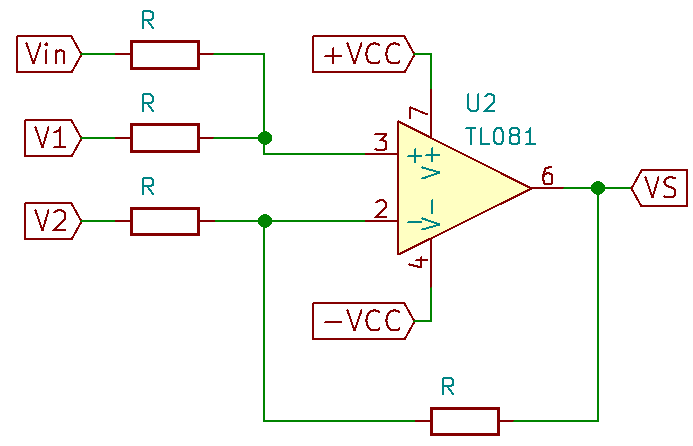
\includegraphics[width=8cm]{images/universel_sommateur.png}
\end{center}

Donner la relation entre $V_S$, $V_1$, $V_2$ et $V_{in}$.

\centerline {\rule{.5\linewidth}{.25pt}} % Horizontal line
%%%%%%%%%%%%%%%%%%%
\textbf{Structure universelle}

Soit la structure suivante, basée sur les montages vus précédemment :

\begin{center}
	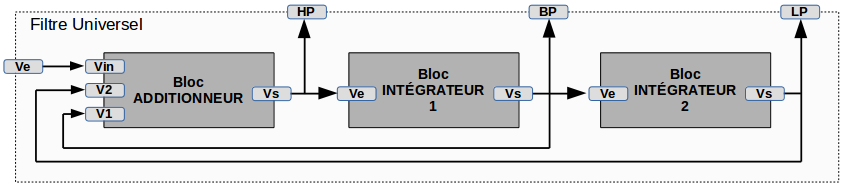
\includegraphics[width=12cm]{images/universel_structure.png}
\end{center}

\begin{enumerate}
	\item Calculer $V_{HP}$ en fonction de $V_{in}$ et des divers composants.	
	\item Calculer $V_{BP}$ et $V_{LP}$.	
	\item Que peuvent signifier les noms donnés aux signaux de sortie ?
\end{enumerate}
}


\encadreTDExo{3.3 - Filtre universel (suite)}{
%%%%%%%%%%%%%%%%%%%
\textbf{Etude du composant UAF42}

On souhaite s'intéresser au composant UAF42, dont quelques pages de documentation technique sont données en annexe.

\begin{enumerate}
	\item Retrouve-t-on la structure étudiée précédemment dans le schéma de la page 1 de la documentation technique ?
	\item Le câblage de la figure 1 de la page 6 de la documentation technique est-il conforme à la structure universelle proposée précédemment ?
	\item Retrouve-t-on la fonction de transfert calculée précédemment ?
	\item Que doivent valoir $R_{F1}$ et $R_{F2}$ pour obtenir une pulsation de coupure de $30~10^3\operatorname{rd/s}$ ?
\end{enumerate}

}

%%%%%%%%%%%%%%%%%%%
\textbf{Bloc intégrateur}

Le montage associé est un amplificateur inverseur. Ainsi, on a : $V_S = V_E \cdot (- Z_C / R)$ avec $Z_C = 1 / (j \cdot \omega (C + C_{out})$.

Ainsi :

$$ \frac{V_S}{V_E} = \frac{- 1}{j \cdot \omega \cdot R_F \cdot (C + C_{out})}$$

\textbf{Transformée de Fourier d'une dérivée}

La dérivée/intégration dans l'espace des fréquences peut s'écrire :

$TF[f'(t)] = \int_{0}^{+\infty} exp(-j \omega t) f'(t) dt$

Par intégration par partie, on obtient :

$TF[f'(t)] = [exp(-j \omega t) f(t)]-{0}^{+\infty} - (-j \omega)  \int_{0}^{+\infty} exp(-j \omega t) f(t) dt$

Ainsi : $TF[f'(t)] = p \cdot TF[f(t)] - f(0)$

\medskip

On peut montrer de la même façon que : $TF[\int_{0}^{t} f(\tau) d\tau] = \frac{1}{j \omega} \cdot TF[f(t)]$

\centerline {\rule{.5\linewidth}{.25pt}} % Horizontal line
%%%%%%%%%%%%%%%%%%%
\textbf{Bloc additionneur}

	L'ALI est en mode linéaire : $V+ = V-$.
	
	Par application du théorème de Millman, on obtient :
	
	$$V+ = \frac{\frac{V_S}{R} + \frac{V_2}{R} }{\frac{2}{R}} $$
	
	$$V- = \frac{\frac{V_{in}}{R} + \frac{V_1}{R}}{\frac{2}{R}}$$

	Ainsi : 
	
	$$V_S = V_{in} + V_1 - V_2$$
	
\centerline {\rule{.5\linewidth}{.25pt}} % Horizontal line
%%%%%%%%%%%%%%%%%%%
\textbf{Structure universelle}

\textbf{Question 1}

	$V_{HP} = V_{in} + V_{BP} + V_{LP}$
	
	Or, $V_{BP} = -\frac{V_{HP}}{j \cdot R_F \cdot C \cdot \omega} $ et $V_{LP} = -\frac{V_{BP}}{j \cdot R_F \cdot C \cdot \omega} = \frac{V_{HP}}{(j \cdot R_F \cdot C \cdot \omega)^2}$
	
	Ainsi :
	
	$$V_{HP} = V_{in} - \frac{V_{HP}}{j \cdot R_F \cdot C \cdot \omega} - \frac{V_{HP}}{(j \cdot R_F \cdot C \cdot \omega)^2}$$
	
	On obtient alors la fonction de transfert suivante :
	
	$$\frac{V_{HP}}{V_{in}} = \frac{(j \cdot R_F \cdot C \cdot \omega)^2}{1 + j \cdot R_F \cdot C \cdot \omega + (j \cdot R_F \cdot C \cdot \omega)^2}$$

	
\centerline {\rule{.3\linewidth}{.25pt}} % Horizontal line
%%%%%%%%%%%%%%%%%%%
\textbf{Question 2}

	$V_{BP} = -\frac{V_{HP}}{j \cdot R_F \cdot C \cdot \omega} $ et $V_{LP} = -\frac{V_{BP}}{j \cdot R_F \cdot C \cdot \omega} = \frac{V_{HP}}{(j \cdot R_F \cdot C \cdot \omega)^2}$
	
	On obtient alors :

	$$\frac{V_{BP}}{V_{in}} = \frac{-j \cdot R_F \cdot C \cdot \omega}{1 + j \cdot R_F \cdot C \cdot \omega + (j \cdot R_F \cdot C \cdot \omega)^2}$$

	Et :

	$$\frac{V_{BP}}{V_{in}} = \frac{1}{1 + j \cdot R_F \cdot C \cdot \omega + (j \cdot R_F \cdot C \cdot \omega)^2}$$


\centerline {\rule{.3\linewidth}{.25pt}} % Horizontal line
%%%%%%%%%%%%%%%%%%%
\textbf{Question 3}
	
	On s'aperçoit que les fonctions de transfert trouvées aux questions précédentes correspondent respectivement à :
	\begin{itemize}
		\item $\frac{V_{HP}}{V_{in}}$ celle d'un filtre passe-haut du second ordre (High Pass)
		\item $\frac{V_{BP}}{V_{in}}$ celle d'un filtre passe-bande (Band Pass)
		\item $\frac{V_{LP}}{V_{in}}$ celle d'un filtre passe-bas du second ordre (Low Pass)
	\end{itemize}

\centerline {\rule{.5\linewidth}{.25pt}} % Horizontal line
%%%%%%%%%%%%%%%%%%%
\textbf{Etude du composant UAF42}

\textbf{Question 1}

Oui, on retrouve l'ensemble des éléments précédents.

\centerline {\rule{.3\linewidth}{.25pt}} % Horizontal line
%%%%%%%%%%%%%%%%%%%
\textbf{Question 2}	

Si on s'intéresse aux équations données à la page 5 de la documentation technique, on retrouve en effet des fonctions de transfert proches de celle calculée précédemment. Avec $s = j \cdot \omega$.	


\centerline {\rule{.3\linewidth}{.25pt}} % Horizontal line
%%%%%%%%%%%%%%%%%%%
\textbf{Question 3}

	D'après la formule en dessous de la figure 1 de la page 6 de la documentation technique, on a :
$\omega_n^2 = \frac{R_2}{R_1} \cdot \frac{1}{R_{F1} \cdot R_{F2} \cdot C_1 \cdot C_2}$.

	On a aussi $C_1 = C_2 = 1\operatorname{nF}$ et $R_1 = R_2$.
	
	On a alors : $$	R_{F1} \cdot R_{F2} = \frac{1}{\omega_n^2 \cdot C_1 \cdot C_2}$$
	
	AN : $R_{F1} \cdot R_{F2} = 1.11 \cdot 10^{9}$
	
	Si on choisit $R_{F1} = R_{F2} = R$, alors $R = 33\operatorname{k\Omega}$



%%%%%%%%%%%%%%%%%%%
%%%%%%%%%%%%%%%%%%%
\encadreTDExo{3.B1 - Impact des ALI}{
On se propose d'étudier le montage suivant : 

\begin{center}
\begin{circuitikz}
	\draw (0,0) node[above]{} ++(1,0) node[ground](GND){}
	node[op amp, noinv input up, anchor=+, fill=blue!10!white](OA){\texttt{AOP1}}
	(OA.-) to[short,-, i<_=$i^-$] ++(0,-1) coordinate(FB) 
	to[R=$R_1$, i=$I_1$] ++(-2,0) to[C=$C$, -o] ++(-2,0) 
	(FB) to[R=$R_2$, *-] (FB -| OA.out) to[short,-, i<_=$I_2$] (OA.out)
	to [short, *-o] ++(1,0) node[above]{};
	\draw (-3,-2.3) edge[<-,color={green!40!black}] (-3, -4);
	\draw (-3,-4.3) to[open,-o] ++(0,0) node[ground](GND){};
	\node[text={green!40!black}] (Ve) at (-3.5,-3.3){$V_E$}; 
	\draw (4.3,-1) edge[<-,color={red}] (4.3, -4);
	\draw (4.3,-4.3) to[open,-o] ++(0,0) node[ground](GND){};
	\node[text={red}] (Vs) at (4.8,-2.7){$V_S$}; 
\end{circuitikz}
\end{center}

\begin{enumerate}
	\item Donnez la fonction de transfert de ce montage dans le cas des hypothèses classiques sur les amplificateurs intégrés (régime linéaire en particulier : $V^+ = V^-$).

	\item Donnez la fonction de transfert de ce même montage en faisant l'hypothèse que la relation qui régit l'amplificateur linéaire est la suivante : $V_S = A_0 \cdot (V^+ - V^-)$. 

	\item Donnez la fonction de transfert de ce même montage en faisant l'hypothèse que la relation qui régit l'amplificateur linéaire est la suivante : $V_S = A(j\omega) \cdot (V^+ - V^-)$. 
	
	On prendra $$A(j\omega) = \frac{A_0}{1 + j \omega / \omega_0}$$
	
	\item Expliquez alors la différence de comportement obtenu entre les 3 modélisations.
\end{enumerate}
}



%%%%%%%%%%%%%%%%%%%
%%%%%%%%%%%%%%%%%%%
\encadreTDExo{3.B2 - Filtre à capacité commutée}{

Nous allons nous intéresser à présent à des filtres dont la fréquence de coupure est pilotable par un signal extérieur.

%%%%%%%%%%%%%%%%%%%%%%%%%%%%%%%%%%%
\textbf{Capacité commutée}

On donne dans un premier temps la structure suivante, dont l'interrupteur $K$ est piloté par le signal de commande ci-dessous :

\begin{center}
	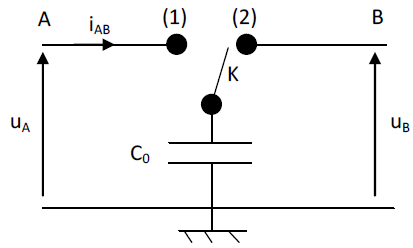
\includegraphics{images/capa_comm.png} 
	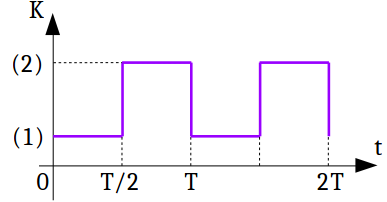
\includegraphics{images/capa_comm_signal.png}
\end{center}


\medskip

\begin{enumerate}
	\item Calculer la charge stockée dans $C_0$ entre les instants 0 et $T/2$, puis entre les instants $T/2$ et $T$.
	\item Quelle quantité de charges passe de A vers B entre les instants 0 et T ?
	\item Calculer alors le courant moyen circulant du point A au point B pendant une période T. 
	\item Donner l'expression de la résistance équivalente $R_{AB}$ vue entre les bornes A et B de cette cellule.
\end{enumerate}

\centerline {\rule{.5\linewidth}{.25pt}} % Horizontal line
%%%%%%%%%%%%%%%%%%%%%%%%%%%%%%%%%%%%%%%%%%%%%%%%%%%%%%%%%%%%%%%%%%
\textbf{Intégrateur à capacité commutée}

On réalise un intégrateur à partir du circuit de la figure 2.

\begin{enumerate}
	\item Donner la fonction de transfert du circuit $T(j\omega) = u_2/u_1$ en fonction de $R_{AB}$ et de $C$.


\begin{center}
	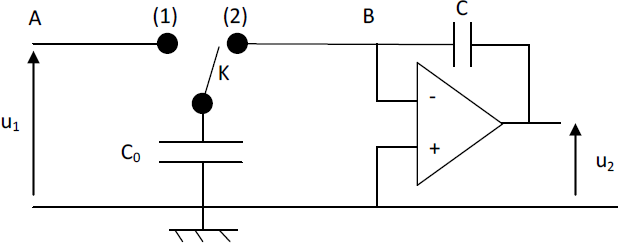
\includegraphics{images/capa_comm_integrateur.png}
\end{center}

	\item Que devient alors la fonction de transfert $T(j\omega{}) = u_2/u_1$ en fonction des éléments du système ($C_0$ et $C$) ?

	\item Quel est l'intérêt d'un tel circuit ?
\end{enumerate}
}

%%%%%%%%%%%%%%%%%%%
\textbf{Bloc additionneur}

\textbf{Question 1}

Pour $0 <= t <= T/2$, on a $u_{C0} = u_A$ et $Q_A = C_0 \cdot u_A$.

Pour $T/2 <= t <= T$, on a $u_{C0} = u_B$ et $Q_B = C_0 \cdot u_B$.


\textbf{Question 2}

$$\Delta{}Q = Q_A - Q_B = C_0 \cdot (u_A - u_B)$$


\textbf{Question 3}

$$i_{AB} = \Delta{}Q / T = C_0 \cdot (u_A - u_B) / T = f \cdot C_0 \cdot (u_A - u_B)$$


\textbf{Question 4}

$$R_{AB} = (u_A - u_B) / i_{AB} = 1 / (f \cdot C_0)$$



\centerline {\rule{.5\linewidth}{.25pt}} % Horizontal line
%%%%%%%%%%%%%%%%%%%
\textbf{Intégrateur à capacité commutée}

\textbf{Question 1}

$$\frac{u_2}{u_1} = \frac{-Z_C}{R_{AB}}$$ avec $Z_C = \frac{1}{j \cdot C \cdot \omega}$


\textbf{Question 2}

$$T(j\omega) = \frac{C_0 \cdot f}{j \cdot C \cdot \omega}$$
	
où $f$ est la fréquence de commutation de l'interrupteur K.


\textbf{Question 3}

Pouvoir piloter la fréquence de transition des intégrateurs.


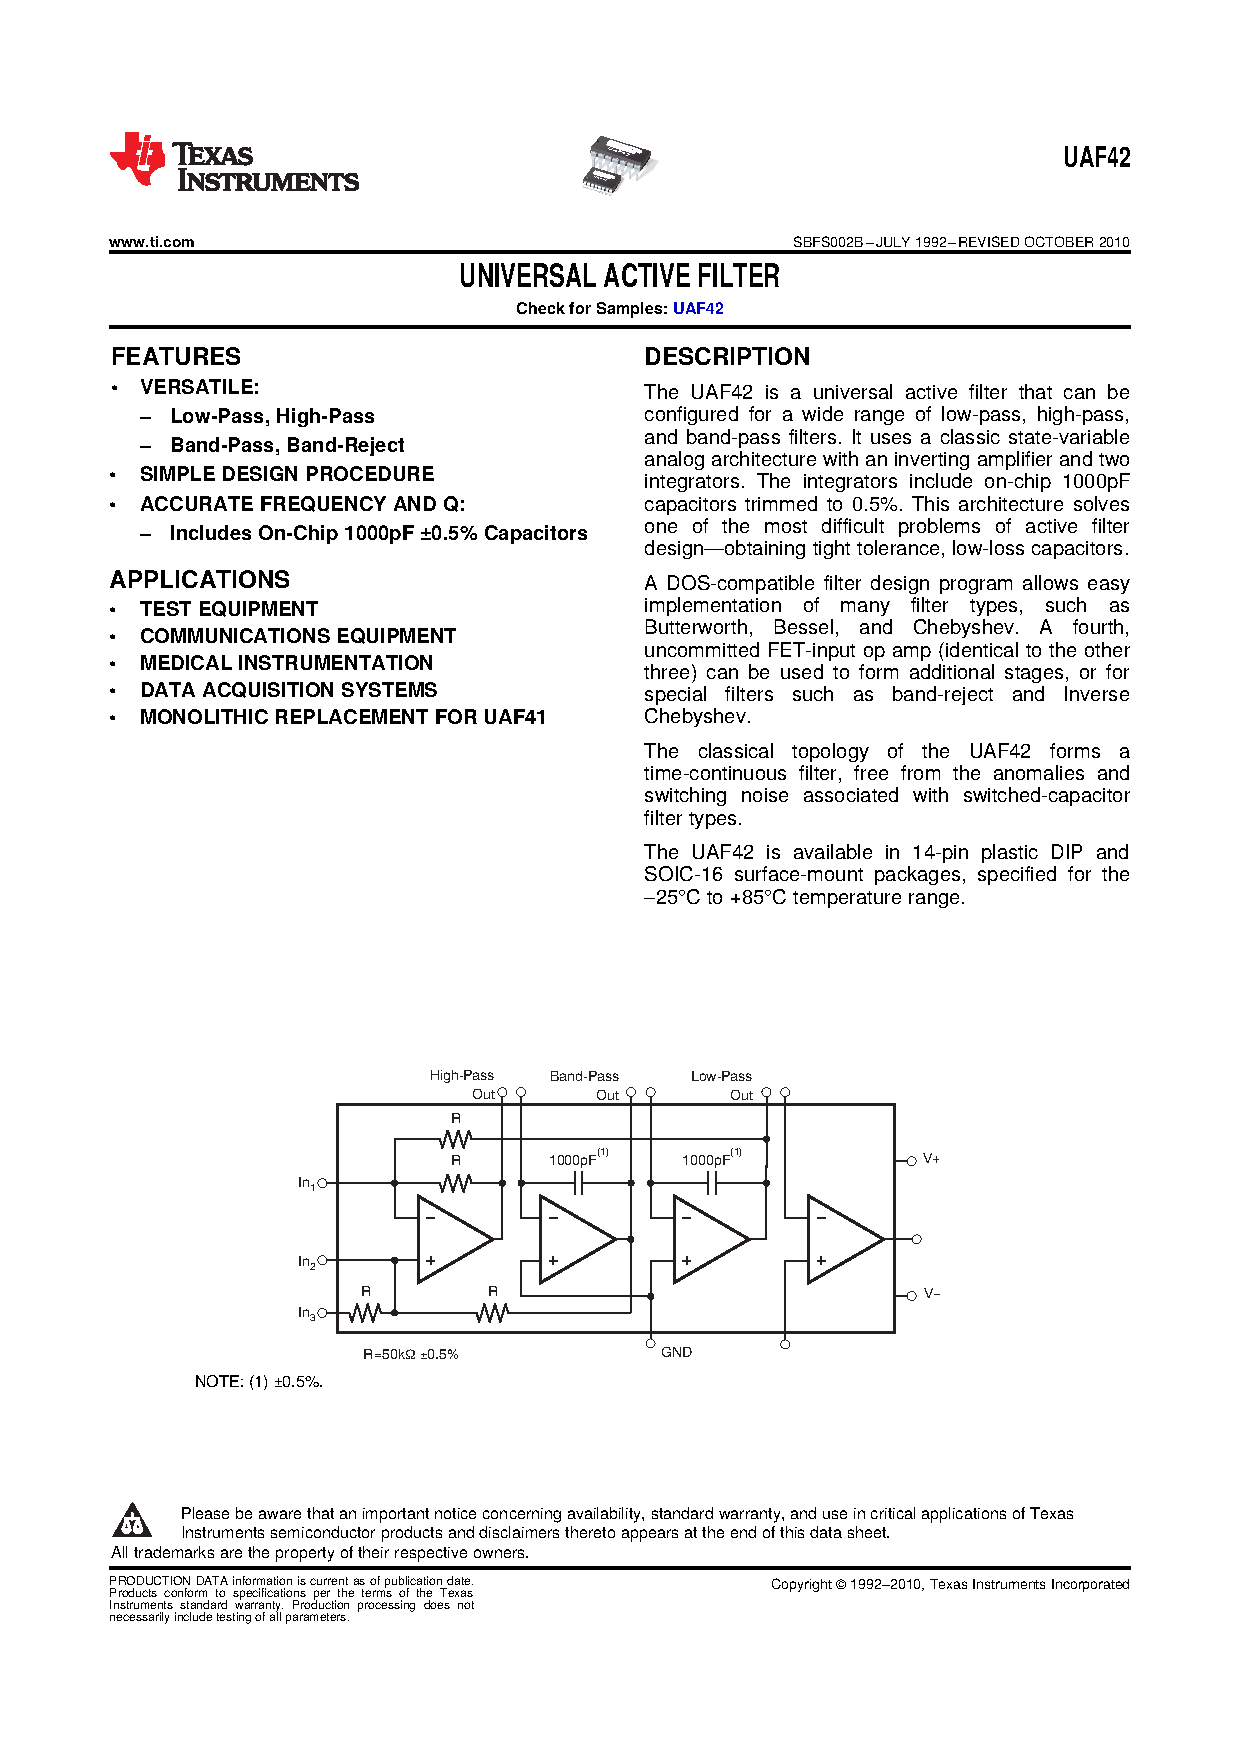
\includepdf[pages=-]{docs/uaf42.pdf}

\end {document}